	\chapter{Convolutional Neural Networks}
	\section{Frequently Asked Questions}

	\resetquestioncounter{}
	\begin{qanda}
		\begin{question}
 What is Computer Vision?
		\end{question}
		\begin{answer}
Computer Vision is a field of Artificial Intelligence that enables computers or systems to derive or extract meaningful information from a digital image or video data and take actions or recommendations based on this information.
		\end{answer}
	\end{qanda}

	\begin{qanda}
		\begin{question}
 What is the Normalization of pixels?
		\end{question}
		\begin{answer}
For most image data, the pixel values are integers with values between 0 and 255. Normalization scales these pixel values between 0 and 1 before modeling.
		\end{answer}
	\end{qanda}

	\begin{qanda}
		\begin{question}
Why should Normalization be performed on pixels?
		\end{question}
		\begin{answer}
Neural networks process inputs using small weight values and inputs with large integer values can disrupt or slow down the learning process, so it is a good practice to normalize the pixels so that the values would range between 0 and 1.
		\end{answer}
	\end{qanda}

	\begin{qanda}
		\begin{question}
How is smoothing performed on images?
		\end{question}
		\begin{answer}
Smoothing an image is required to reduce noise and blur the false edges. Smoothing is usually performed using Gaussian Blur. Gaussian filtering is highly effective at removing noise from the image. We can use the below code to perform Gaussian Blur.

		\begin{code}[\codenumbering]{}
			\codeitemnonumber blur\_image = cv2.GaussianBlur(original\_image, (5,5), 0)
		\end{code}
		\end{answer}
	\end{qanda}

	\begin{qanda}
		\begin{question}
Will the images always be provided in zip file format?
		\end{question}
		\begin{answer}
The image data sets are usually provided in the following formats:

	\begin{bulletedlist}
		\item {\bfseries Folders/Directories}: The whole data set can be given in a single directory or a zip file which can be extracted to get a directory. This directory can contain sub-folders like training and testing. The training and testing folders may contain individual sub-folders for each category of image. The whole structure can be observed in the \figurename~\ref{fig:cnnimagesinfiles}.
		\item {\bfseries TensorFlow data sets}: The data sets can be loaded from as shown in \figurename~\ref{fig:cnntensorflowdataset}.
		\item {\bfseries numpy arrays}: The images can also be given as numpy arrays and the labels to the corresponding images can be given in a CSV file.  The images that are converted into numpy arrays can be given in \textcode{images.npy} file and the labels corresponding to each image can be given in the \textcode{labels.csv file}.  The \textcode{np.load()} function can be used to read the numpy arrays and the \textcode{pd.read\_csv()} function from pandas can be used to read the \textcode{csv} file as shown in \figurename~\ref{fig:cnnnumpyarraydataset}.
	\end{bulletedlist}
		\end{answer}
	\end{qanda}

	\begin{figure}[h]
		\centering
		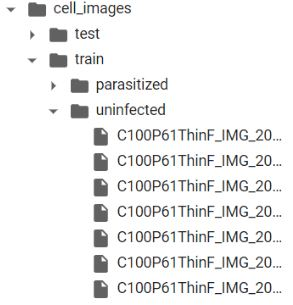
\includegraphics[height=2in]{cnnimagesinfiles}
		\caption[Cross validation]{Cross validation.}
		\label{fig:cnnimagesinfiles}
	\end{figure}

	\begin{figure}[h]
		\centering
		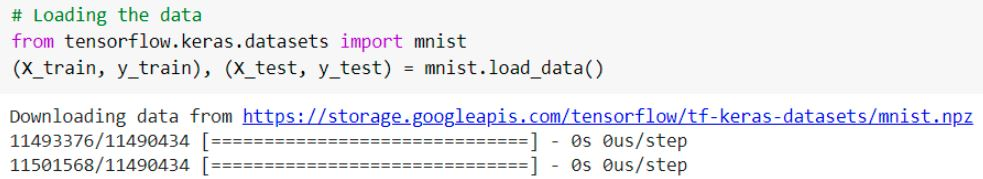
\includegraphics[width=\textwidth-1in]{cnntensorflowdataset}
		\caption[Loading a TensorFlow image data set]{Loading a TensorFlow image data set.}
		\label{fig:cnntensorflowdataset}
	\end{figure}

	\begin{figure}[h]
		\centering
		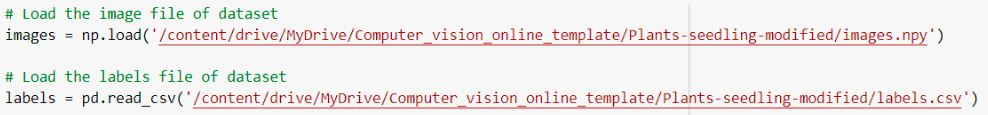
\includegraphics[width=\textwidth]{cnnnumpyarraydataset}
		\caption[Numpy array loading of image data set]{Numpy array loading of image data set.}
		\label{fig:cnnnumpyarraydataset}
	\end{figure}

	\begin{qanda}
		\begin{question}
Do we need to split the image data into train and test sets before pre-processing?
		\end{question}
		\begin{answer}
The splitting of image data should be performed before any operations or pre-processing steps on images.  One way is to divide the data set into two subsets:
	\begin{numberedlist}
		\item Training set: a subset to train a model.
		\item Test set: a subset to test the model.
	\end{numberedlist}

Separating the data enables you to evaluate your model generalization capabilities and have an idea of how it would perform on unseen data.  Good performance on the test set is a useful indicator of good performance on new data in general, assuming that:
	\begin{bulletedlist}
		\item The samples were drawn independently and at random from the distribution to create the test set.
		\item The test set is large enough.	
	\end{bulletedlist}

The second way is to divide the data set into three subsets:
	\begin{numberedlist}
		\item Training set: a subset to train a model.
		\item Validation set: a subset to validate and tune our model.
		\item Test set: a subset to test the model.
	\end{numberedlist}
		\end{answer}
	\end{qanda}

	\begin{qanda}
		\begin{question}
What is the difference between MNIST and Fashion MNIST data sets that are used in the course?
		\end{question}
		\begin{answer}
The MNIST data consists of images of 10 handwritten digits from 0 to 9, and this data set can be directly loaded using the \textcode{load\_data()} function of TensorFlow.  Whereas, Fashion MNIST can also be loaded using the same \textcode{load\_data()} function, it consists of fashion images like shoes, shirts, etc belonging to 10 different categories.
		\end{answer}
	\end{qanda}

	\begin{qanda}
		\begin{question}
What is the difference between \textcode{resize()} and \textcode{reshape()} functions (in context of images)?
		\end{question}
		\begin{answer}
The \textcode{reshape()} function changes the shape only and not the number of pixels.  For example, the image of size 6 x 4 can be reshaped into 12 x 2.  Here we did not change the number of pixels.  But an image of 6 x 6 can be resized into 10 x 10 using the resize function.  Here the number of pixels are increased.
		\end{answer}
	\end{qanda}

	\begin{qanda}
		\begin{question}
Which function can be used to get the names of labels that are encoded using an encoder?
		\end{question}
		\begin{answer}
The \textcode{inverse\_transform()} function can be used to decode the labels from the encoded vectors.  For example: if a label ``car'' is encoded using a label binarizer into an array of [0,0,1] then \textcode{inverse\_transform()} can be used to get the label name from this array.
		\end{answer}
	\end{qanda}

	\begin{qanda}
		\begin{question}
How to unzip a zipfile in Google Colab?
		\end{question}
		\begin{answer}
The unzip command can be used to unzip the file in Google Colab.
		\begin{code}[\codenumbering]{}
			\codeitemnonumber !unzip ``path to the file''
		\end{code}
		\end{answer}
	\end{qanda}

	\section{Introduction}

Convolution neural networks are a special type of neural network designed to work with image data.  CNNs use convolutional layers hidden layers which perform convolution operations. They have some different characteristics to artificial neural networks.
	\begin{bulletedlist}
		\item Unlike ANNs, CNNs capture the spatial structure of the image.
		\item CNNs follow the concept of parameter sharing i.e. one filter is applied over the whole image, because of which they are much more computationally efficient.
		\item The first part in this architecture is the convolutional layer followed by the pooling layer and the second part is the fully connected layer.  This whole architecture is called a convolutional neural network.
	\end{bulletedlist}

	\begin{figure}[h]
		\centering
		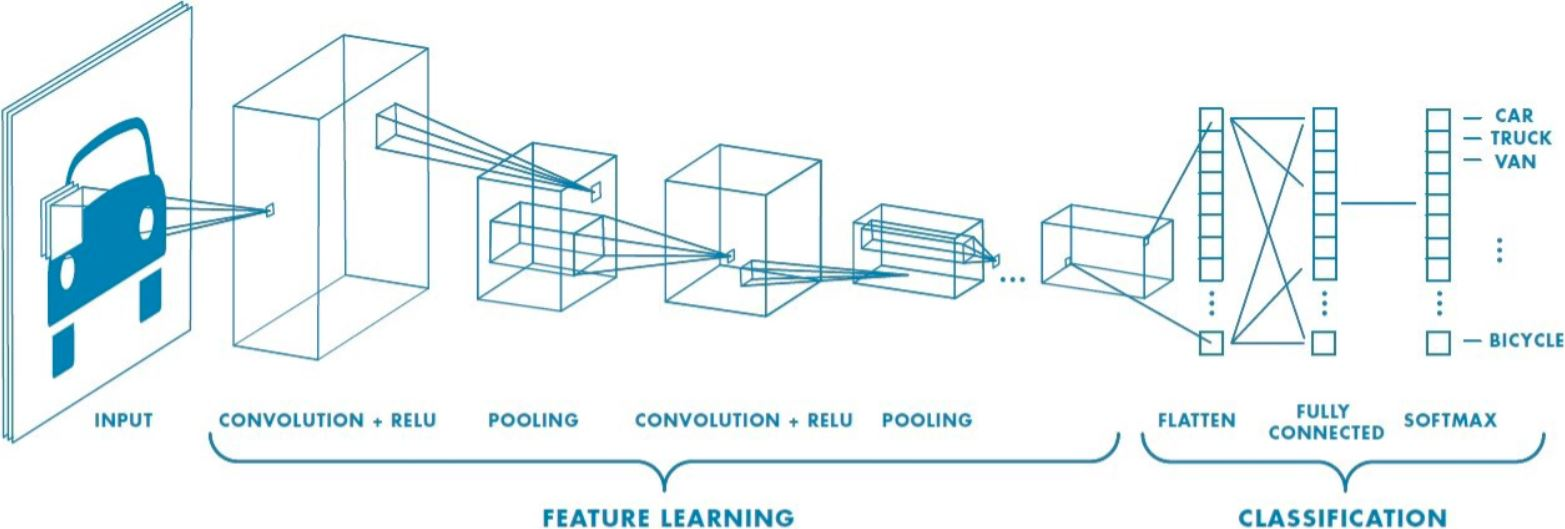
\includegraphics[width=\textwidth]{convolutionneuralnetwork}
		\caption[Convolution neural network]{Convolution neural network.  Image source \href{https://towardsdatascience.com/a-comprehensive-guide-to-convolutional-neural-networks-the-eli5-way-3bd2b1164a53}{toward data science}.}
		\label{fig:convolutionneuralnetwork}
	\end{figure}

	\section{Convolutional Layer - Filter/Kernel}
	\begin{bulletedlist}
		\item A convolution operation uses a small array of numbers called a filter/kernel on the input image.
		\item Each filter is designed to identify a specific feature in the input space of the image, such as horizontal edges, vertical edges etc.
		\item A CNN is able to successfully capture the spatial and temporal dependencies in an image through the application of relevant filters.
		\item The role of the CNN is to reduce the images into a form which is easier to process, without losing features which are important for getting a good prediction.
		\item The convolution is performed as shown in \figurename{}s~\ref{fig:convolutionoperationstepsa} and~\ref{fig:convolutionoperationstepsb}.
	\end{bulletedlist}

	\section{Pooling layer in CNNs}

	\begin{bulletedlist}
		\item After a convolution operation, we usually perform pooling to reduce the dimensions of the feature map.
		\item It enables us to reduce the number of parameters, which both reduces the training time and the over fitting.
		\item Pooling layers down sample each feature map independently, reducing the height and width, but keeping the depth same.
		\item There are two types of pooling - Max and Average.  Max pooling just takes the maximum value whereas average pooling takes the average value in the pooling window (see \figurename~\ref{fig:poolingtypes}).
		\item Contrary to the convolution operation, pooling has no parameters.
	\end{bulletedlist}

	\begin{figure}[h]
		\centering
		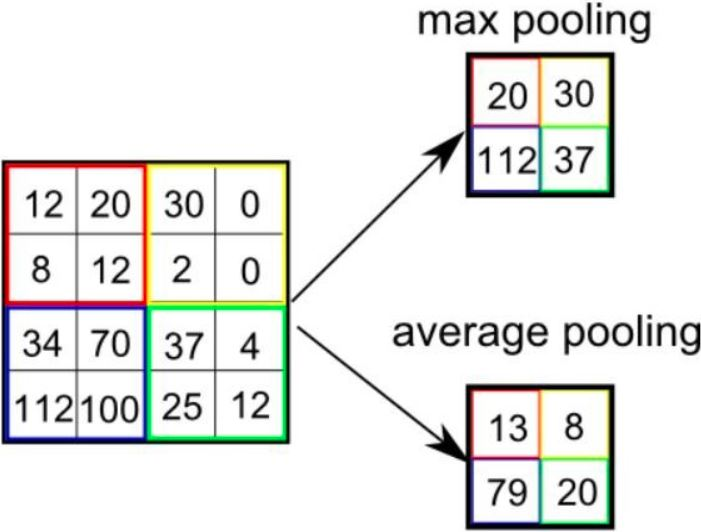
\includegraphics[height=1.5in]{poolingtypes}
		\caption[Types of pooling]{Types of pooling.}
		\label{fig:poolingtypes}
	\end{figure}

	\section{Padding and Stride in CNNs}
	\begin{bulletedlist}
		\item Stride specifies how much we move the filter at each step. By default the value of the stride is 1 and is represented by the first figure
		\item We can also increase the value of stride if we want less overlap between the filters. It also makes the resulting feature map smaller since we are skipping over some locations.
		\item The second figure demonstrates the stride 2.
	\end{bulletedlist}

We see that after using stride, the size of the feature map is smaller than the input. If we want to maintain the same dimensions, we can use padding to surround the input with zeros.  In the following, refer to \figurename~\ref{fig:paddingandstrideincnn}.

	\begin{bulletedlist}
		\item The grey area around the input in the third figure is the padding.
		\item We either pad with zeros or the values on the edge, to match the dimensions of the feature map with the input.
		\item Padding is commonly used in CNNs to preserve the size of the feature maps, otherwise they would shrink at each layer, which is not desirable.
	\end{bulletedlist}

	\begin{figure}[h]
		\centering
		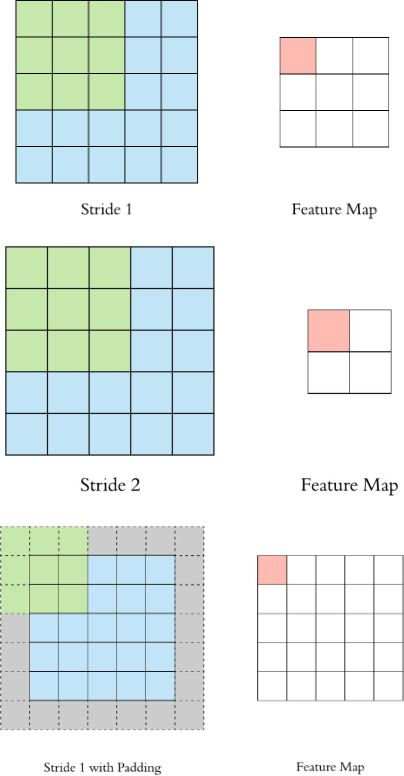
\includegraphics[height=2.5in]{paddingandstrideincnn}
		\caption[Padding and stride in CNNs]{Padding and stride in CNNs.}
		\label{fig:paddingandstrideincnn}
	\end{figure}

